\section{Seasonal adjusted fits for pH and temperature }

Linear regression is not suitable for analyzing seasonal data due to its
assumption of constant variance and independence of observations, which are
often violated in seasonal time series. Seasonal data typically exhibit
patterns that repeat at regular intervals over time, leading to violations of
the independence assumption. Moreover, the variance of the data may not be
constant across different seasons, violating the assumption of constant
variance. These violations can result in biased parameter estimates and
inaccurate predictions when using linear regression models to analyze seasonal
data. To account for seasonality in data, more appropriate methods such as
seasonal decomposition or time series models like SARIMA (Seasonal
Autoregressive Integrated Moving Average) should be employed, which explicitly
capture the seasonal patterns and dependencies present in the data. However,
the presence of missing data make them impractical to use in this study.

Another possibility to obtain the long-term trend of the data is to remove the
seasonal component from the time series. This can be done by fitting a
sinusoidal function to the data and subtracting the fit from the original time
series. Indeed, one can directly fit a sinusoidal function with a linear
component to the data, which can be expressed as:

\begin{equation}
    f(t) = A \sin(\omega t + \phi) + Bt  + C
\end{equation}

where $A$ is the amplitudes of the sine function, $\omega$ is the angular
frequency, $\phi$ is the phase shift, $B$ is the slope of the linear component
and $C$ is the offset. The angular frequency is related to the period of the
function by $\omega = 2\pi/T$, where $T$ is the period. The optimal values for
the parameters were found by minimizing the mean squared error between the
seasonally adjusted data and the fit. The optimal period was found by
minimizing the mean squared error between the seasonally adjusted data and the
fit for different periods. The optimal period was found to be $T=1.006$ for pH
and $T=1.0$ for temperature. The optimal fits are shown in
\cref{fig:seasonally_adjusted_fit_pH,fig:seasonally_adjusted_fit_T}.

\begin{figure}[H]
    \centering
    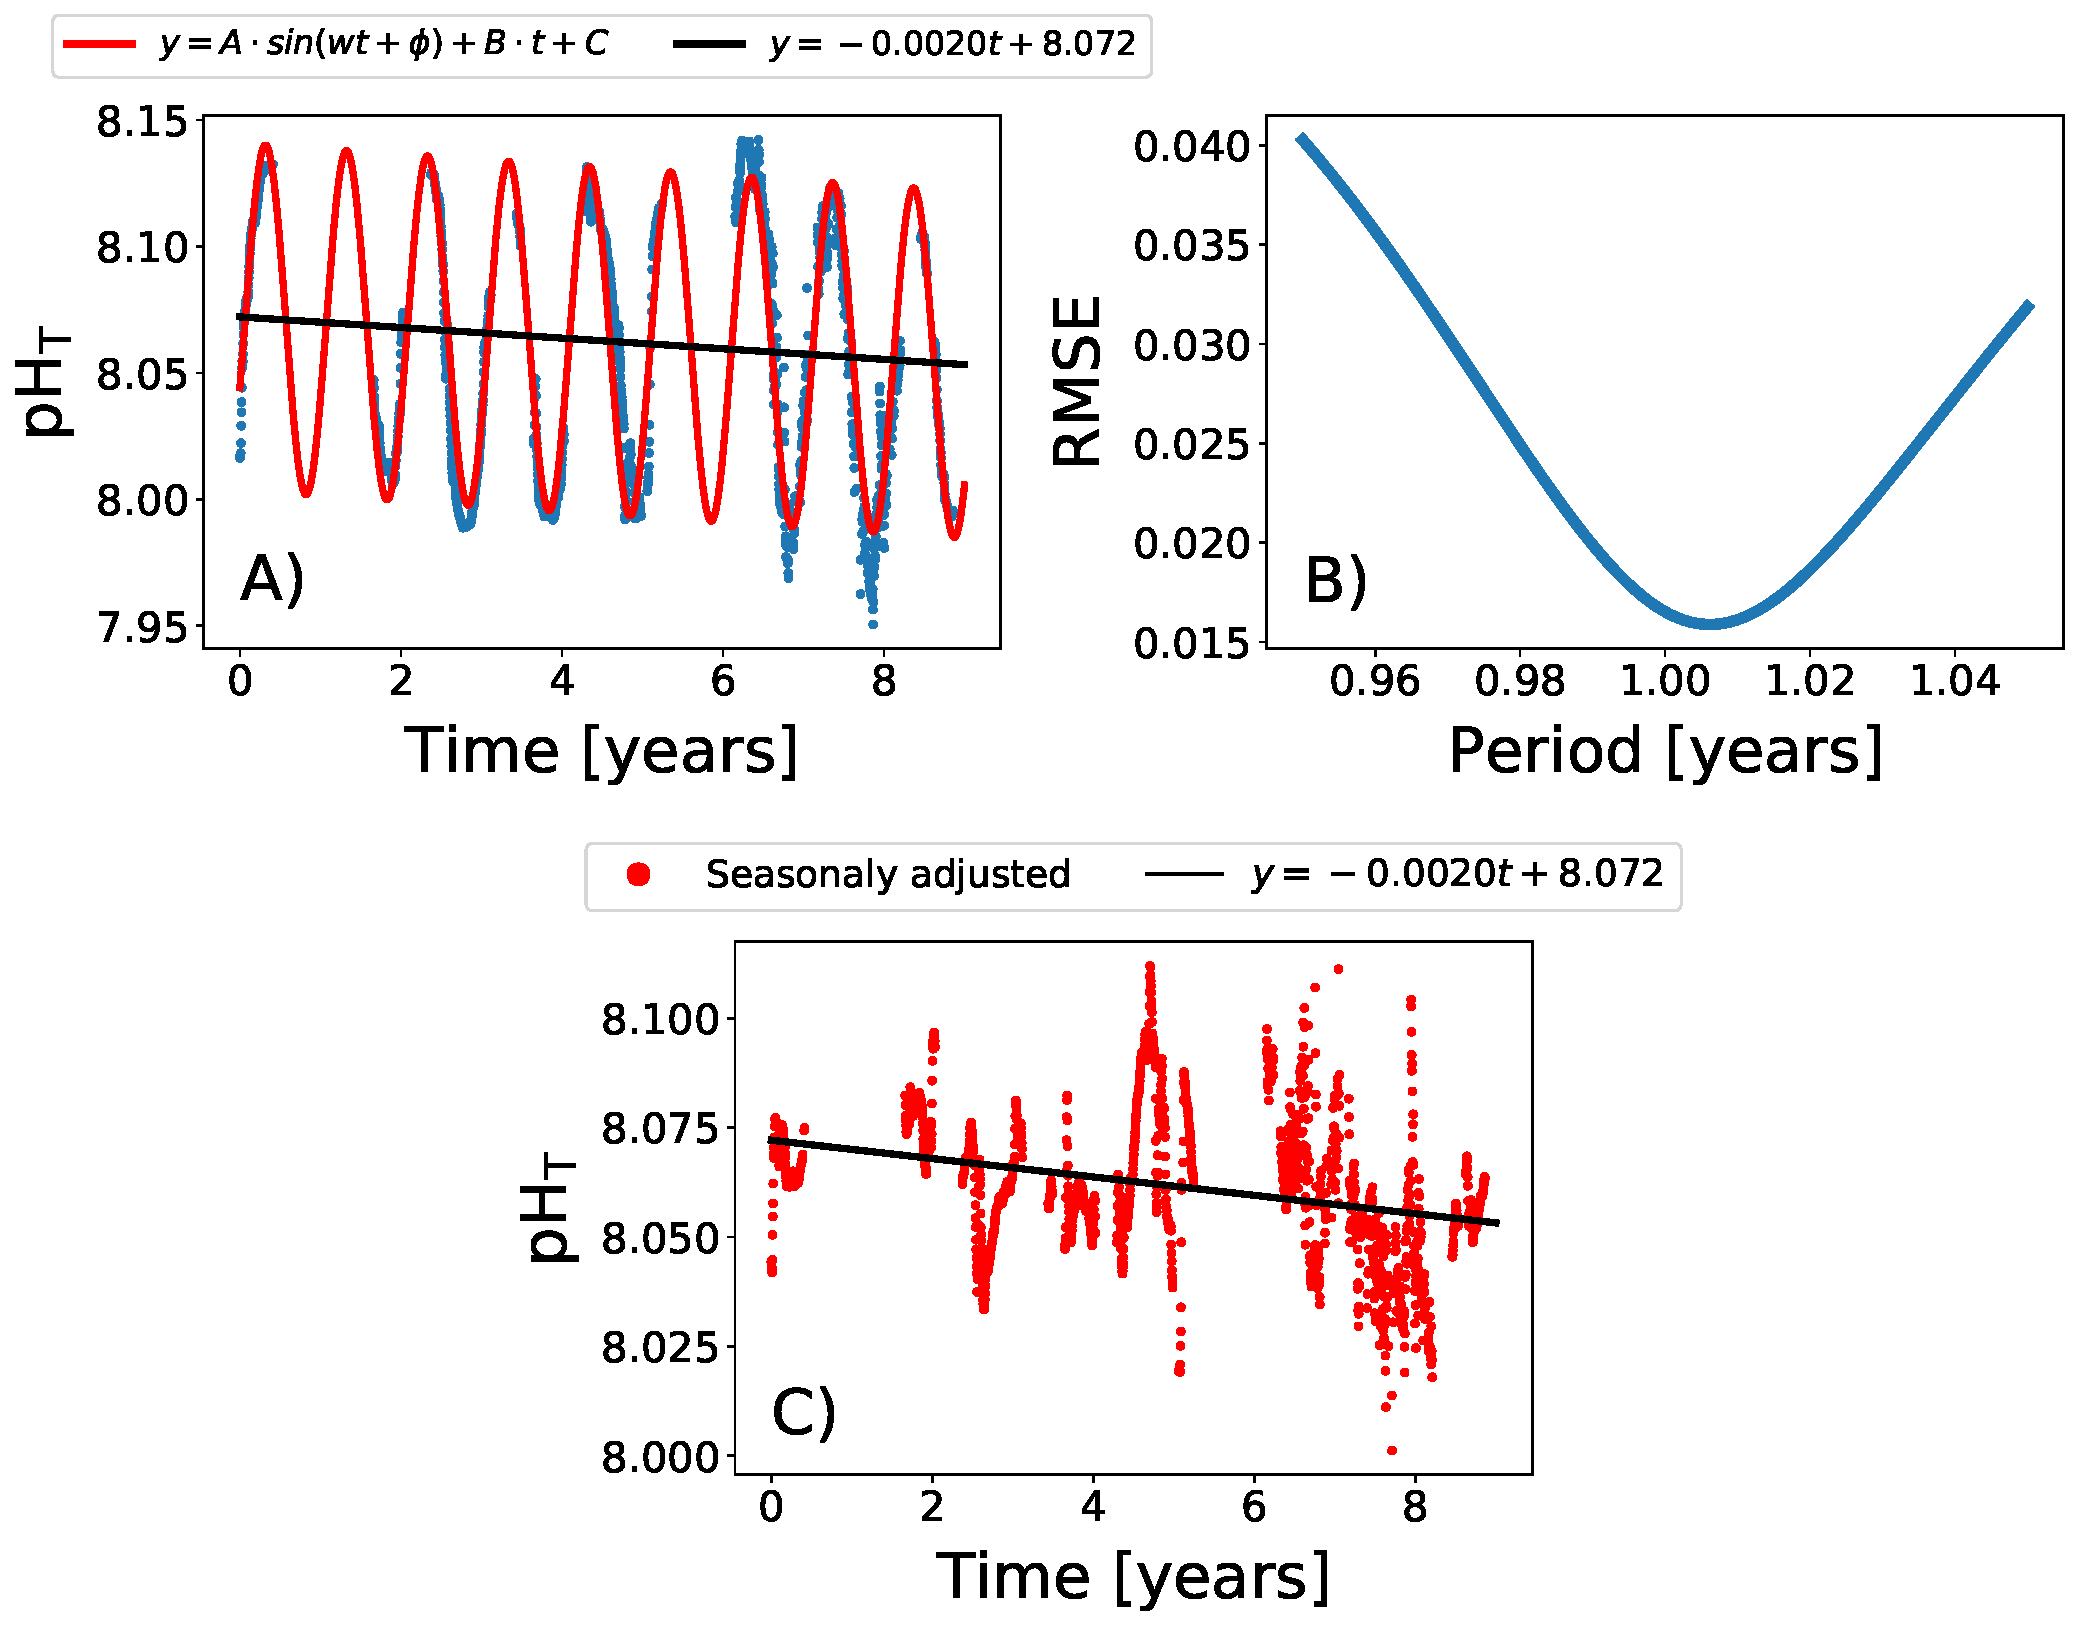
\includegraphics[width=\textwidth]{Figures/Trend_seasonality_pH.pdf}
    \caption{Seasonally adjusted fit to reconstructed and measured pH data.
        A) Full fit of \textcolor{blue}{Eq. (1)} with $A=0.0686 \pm 0.0005$,
        $B=-0.0020
            \pm 0.0002$, $\phi=-6.704 \pm 0.008$,  $C=8.0721 \pm 0.0008$. B)
        Optimal period
        ($T=1.006$, $\omega=2\pi/T$) found to fit the data. C) Linear
        regression to the
        seasonal adjusted data. }
    \label{fig:seasonally_adjusted_fit_pH}
\end{figure}

\begin{figure}[H]
    \centering
    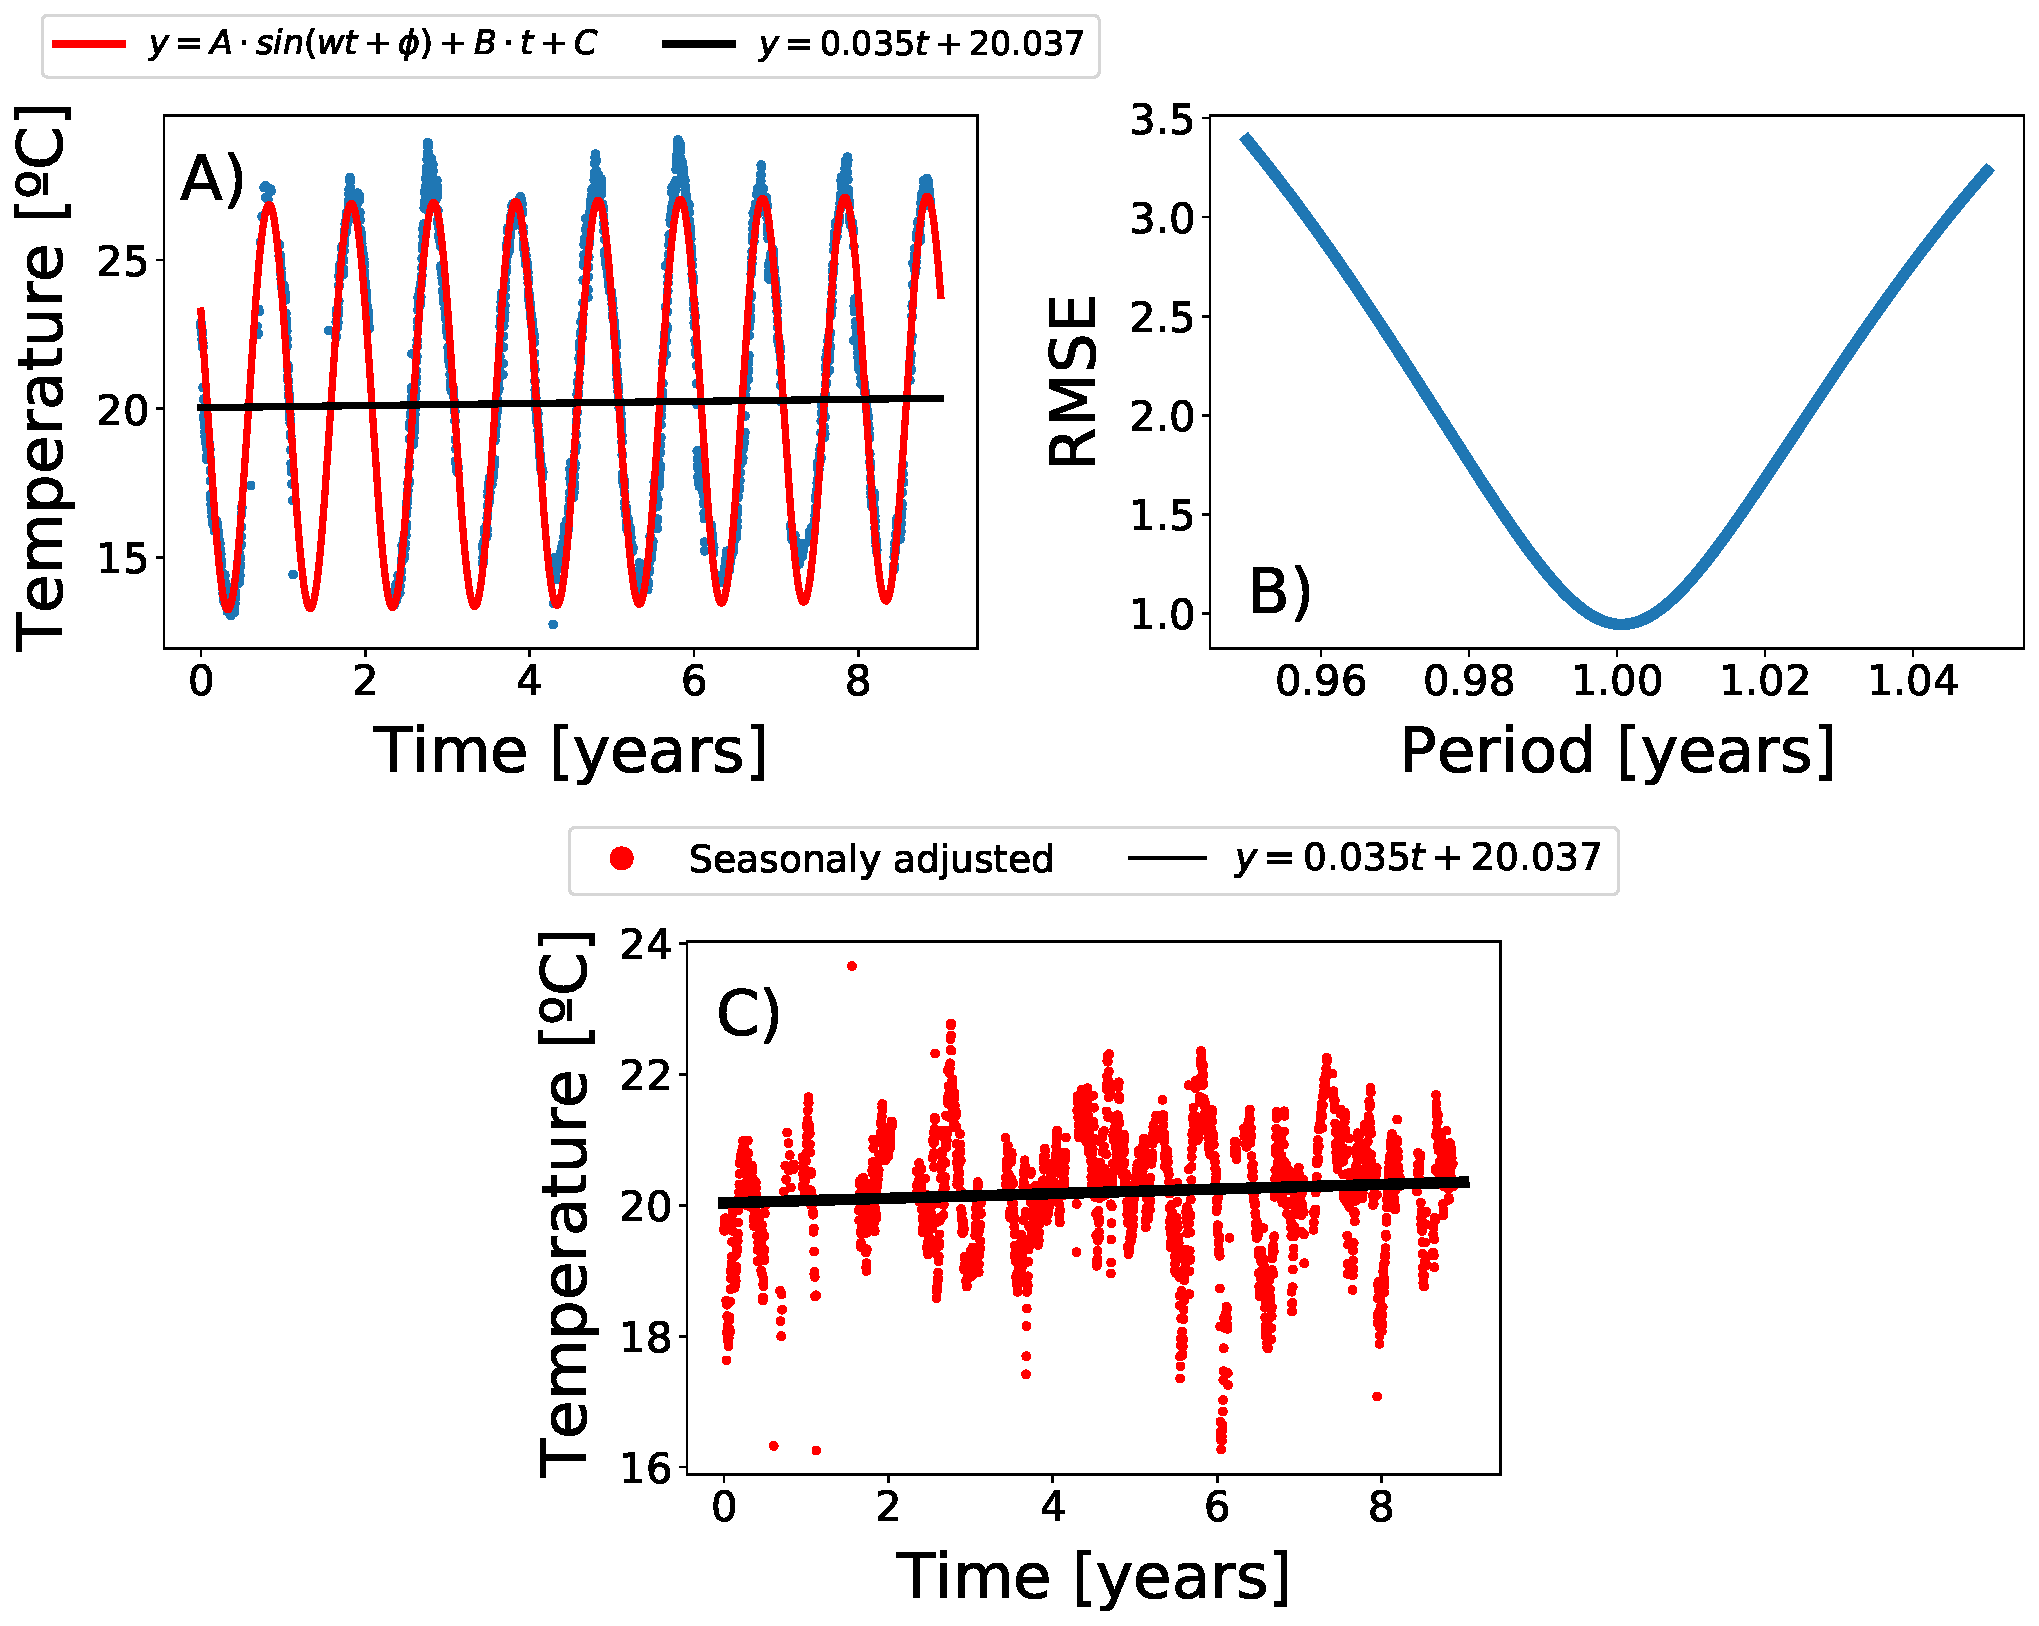
\includegraphics[width=\textwidth]{Figures/Trend_seasonality_T.pdf}
    \caption{Seasonally adjusted fit to reconstructed and measured
        temperature data. A) Full fit of \textcolor{blue}{Eq. (1)} with
        $A=6.792 \pm
            0.029$, $B=-0.0353 \pm 0.0080$, $\phi=-3.6396 \pm 0.0040$,
        $C=20.037 \pm
            0.043$. B) Optimal period ($T=1.0$, $\omega=2\pi/T$) found to fit
        the data. C)
        Linear regression to the seasonal adjusted data.}
    \label{fig:seasonally_adjusted_fit_T}
\end{figure}

\section{Total alkalinity in the Bay of Palma}

\begin{figure}[H]
    \centering
    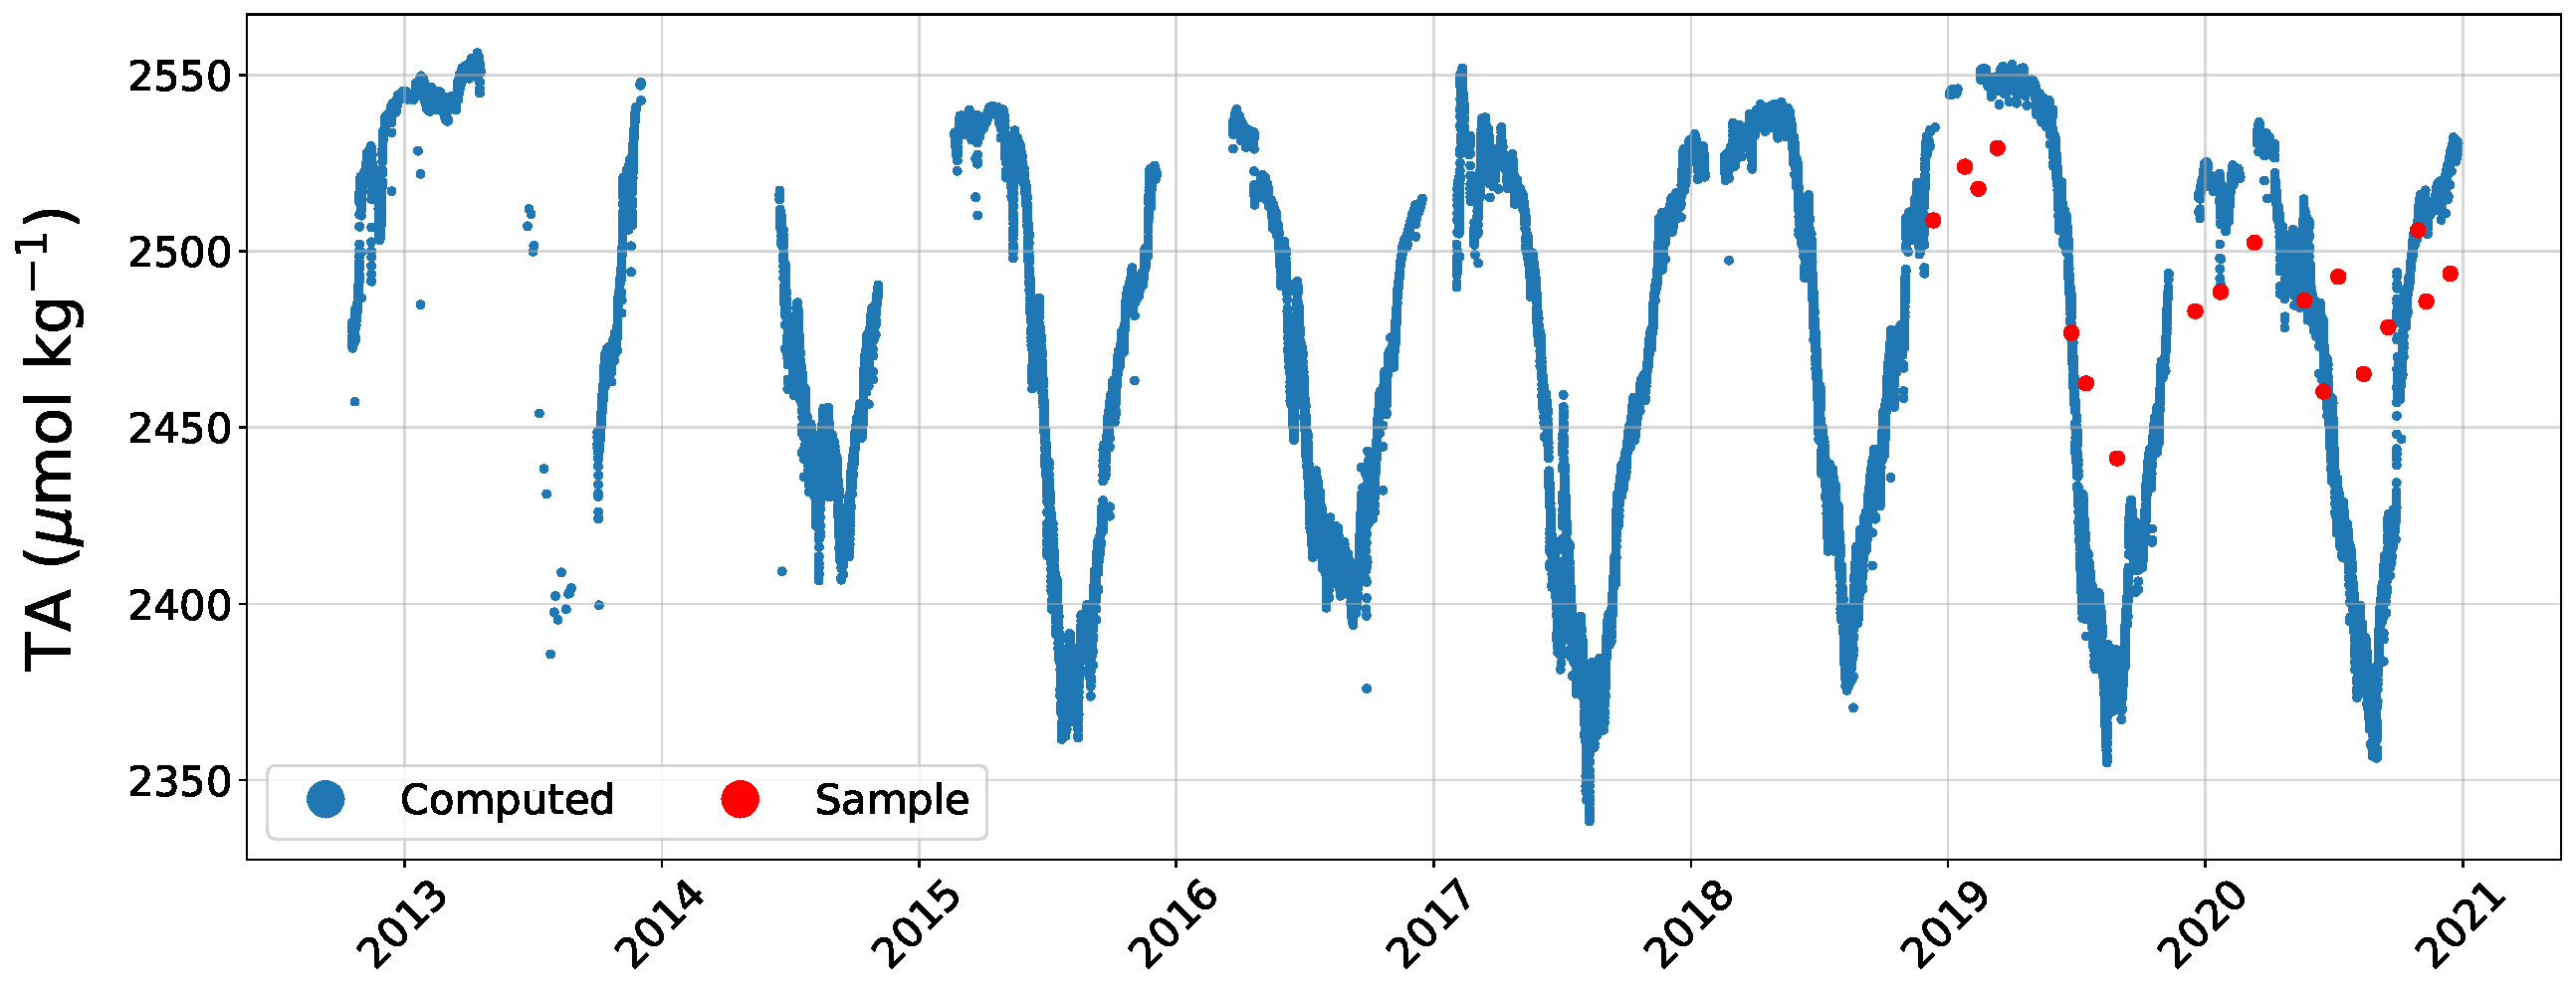
\includegraphics[width=\textwidth]{Figures/S1.pdf}
    \caption{Total alkalinity in ${\mu \textrm{mol\,kg}^{-1}}$ calculated
        values (blue dots) and concentrations obtained from samples (red dots)
        in the
        Bay of Palma.}
    \label{fig:S1}
\end{figure}
